\chapter{Recurrent Restricted Kernel Machines for Time-series Forecasting}\label{cha:rrkm}

\section{Introduction}
In~\cite{suykensdeep2017}, Suykens proposed a new framework called Restricted Kernel Machines (RKM), which provides a representation of kernel methods with visible and latent variables. This representation has an objective function that is similar to the energy function of Restricted Boltzmann Machines (RBM), thus linking kernel methods with RBMs.
Training and prediction requires characterizing the stationary points for the unknowns in the objective. This in turn provides the training and prediction schemes in the kernel methods setting.
Restricted Kernel Machines have been previously extended for different tasks such as classification~\cite{suykensdeep2017}, generation~\cite{GENRKM, st_rkm} and outlier detection~\cite{TONIN2021661}.
We further extend the RKM framework to time series modeling by introducing a temporal correlation on the latent variables which provides powerful representation learning capabilities, and a novel forecasting method. The formulation draws connections with kernel autoregressive models~\cite{KALLAS20133053} and Temporal Restricted Boltzmann Machines (TRBM)~\cite{sutskeverRecurrentTemporalRestricted,osogamiBoltzmannMachinesTimeseries2019}, which are explored in the next sections.

% For an excellent survey of Energy-based Models and Temporal Restricted Boltzmann Machines (TRBM) for time-series modeling see~\cite{osogamiBoltzmannMachinesEnergybased2019},~\cite{osogamiBoltzmannMachinesTimeseries2019}. We draw connections of our model with TRBM in the following section.

% Introduction to dynamical systems modeling/time-series, it's importance and use cases

% Use of latent variable models in the above context

% RKM in context of latent variable models and previous studies in generation and disentanglement.

% Contributions of the current paper: highlight the difference with temporal RBMs which requires binary inputs/latent variables or real-valued inputs/binary latent variables.

% \section{Related Works}~\label{sec:related_works}
% Excellent review of Energy-based Models and Temporal Restricted Boltzmann Machines (TRBM) for time-series modeling~\cite{osogamiBoltzmannMachinesEnergybased2019},~\cite{osogamiBoltzmannMachinesTimeseries2019}

% Introduction to RKMs [Johan's papers]

% Great survey of Variational Auto-Encoders for Dynamical systems modeling~\cite{girinDynamicalVariationalAutoencoders2021}

\section{Recurrent Restricted Kernel Machines }
% In this section, we first propose the objective function and explain how it can be used for training the model. Next, we discuss its use for further predictions.

\subsection{Training}~\label{sec:training}
Our main objective is to capture the dynamics of a training data set $\mathcal{X}_T$ containing $T$ time steps $\{\mathbfit{x}_{t}\}_{t=1} ^{T} \subset{\mathscr{X}}$.
We define a feature map\footnote{Throughout our discussion, we assume that the feature vectors are centered in the feature-space \emph{i.e.} $\bar{\phi}(\mathbfit{x}) = \phi(\mathbfit{x}) - \mu_{\phi}$ with $\mu_{\phi} = \mathbb{E}_{\mathbfit{\xi}\mathcal{\sim X}}\left[\phi(\mathbfit{\xi})\right]$.
Using an implicit formulation, it suffices to notice that $\langle\bar{\phi}(\mathbfit{x}), \bar{\phi}(\mathbfit{y}) \rangle_{\mathscr{H}} = \langle\phi(\mathbfit{x}) - \mu_{\phi}, \phi(\mathbfit{y}) - \mu_{\phi} \rangle_{\mathscr{H}} = \langle\phi(\mathbfit{x}), \phi(\mathbfit{y})\rangle_{\mathscr{H}} - \langle\mu_{\phi}, \phi(\mathbfit{y})\rangle_{\mathscr{H}} - \langle\phi(\mathbfit{x}), \mu_{\phi})\rangle_{\mathscr{H}} + \langle\mu_{\phi}, \mu_{\phi}\rangle_{\mathscr{H}} = k(\mathbfit{x},\mathbfit{y}) - \mathbb{E}_{\mathbfit{\xi}\mathcal{\sim X}}\left[k(\mathbfit{\xi},\mathbfit{y})\right] - \mathbb{E}_{\mathbfit{\zeta}\mathcal{\sim X}}\left[k(\mathbfit{x},\mathbfit{\zeta})\right] + \mathbb{E}_{\mathbfit{\xi},\mathbfit{\zeta}\mathcal{\sim X}}\left[k(\mathbfit{\xi},\mathbfit{\zeta})\right]$.
In practice, we can compute statistics on $\mathcal{X}_T$.} $\phi: \mathscr{X} \rightarrow \mathscr{H}$ with $\mathscr{H}$ a (possibly infinite dimensional) Reproducing Kernel Hilbert Space (RKHS; see~\cite{scholkopf1997kernel} for more details).
Such a feature map could be constructed explicitly or implicitly via a kernel function $ k(\mathbfit{x},\mathbfit{y}) : \mathscr{X}^2 \rightarrow \mathbb{R} : \left(\mathbfit{x},\mathbfit{y} \right) \mapsto \langle\phi(\mathbfit{x}), \phi(\mathbfit{y})\rangle_{\mathscr{H}}$.
We also define a linear operator\footnote{The linear operator $\mathbfit{V}$ is often referred to as a \emph{matrix} as it only exists explicitly in the case of finite dimensional Hilbert spaces $\mathscr{H}$.
It then takes the form $\mathbfit{V} \in \mathbb{R}^{\mathrm{dim}(\mathscr{H}) \times s}$ and $\mathbfit{V}^* = \mathbfit{V}^{\top}$.} $\mathbfit{V}:\mathbb{R}^s \rightarrow \mathscr{H}$ with $s \leq T$ and it's adjoint $\mathbfit{V}^\star$.
Each datapoint $\mathbfit{x}_t$ will be associated to a latent variable $\mathbfit{h}_{t} \in \mathbb{R}^s$ through a pairing term $\langle \phi\left(\mathbfit{x}_t\right), \mathbfit{V} \mathbfit{h}_t \rangle_{\mathscr{H}}$.
To also capture time dependence, we only add one extra term compared to the original RKM framework~\cite{suykensdeep2017}: time correlation in the latent space using a set of non-zero lag-dependent coefficients $\mathcal{A}_T = \left\{ a_{t,l} \left| 1 \leq t  \leq T \;\text{and}\; 0 \leq l < p \right.\right\}$ with $p \in \mathbb{Z}^{+}$ a lag parameter (other coefficients are assumed to be $0$).
Then consider the following objective function with diagonal matrix $\mathbfit{\Lambda}$:
\abovedisplayshortskip.50ex
\belowdisplayshortskip.50ex
\begin{align}
	J_T(\mathbfit{V},\mathcal{H}_T,\mathcal{X}_T) =  \sum_{t=1}^{T} \Big[ & -\xoverbrace{ \langle \phi(\mathbfit{x}_{t}) , \mathbfit{V} \mathbfit{h}_{t} \rangle_{\mathscr{H}} }^{\text{feature-space pairing}} - \xoverbrace{\sum_{l=0}^{p} a_{t,l} \mathbfit{h}_{t-l} ^{\top}  \mathbfit{h}_{t}}^{\text{temporal covariance}} \nonumber \\
	                                                                & +\underbrace{\frac{1}{2} \left( \mathbfit{h}_{t}^{\top}\mathbfit{\Lambda}\mathbfit{h}_{t} + \Vert \phi(\mathbfit{x}_{t})\Vert_{\mathscr{H}}^{2} \right)\Big] +  \frac{1}{2}\mathrm{Tr}\left(\mathbfit{V}^*\mathbfit{V}\right)}_{\text{regularization}}.
	\label{eq:rrkm_training_objective}
\end{align}
% 
% \begin{align}
% 	J(\mathbfit{V};\mathbfit{h}_t;\mathbfit{x}_t) =  -\xoverbrace{\phi(\mathbfit{x}_t) ^{\top} \mathbfit{V} \mathbfit{h}_t}^{\text{(spatial) pairing}} - \xoverbrace{\sum_{k=0}^{p} a_{t,l} \mathbfit{h}_{t-k} ^{\top}  \mathbfit{h}_{t}}^{\text{temporal correlation}} \\
% 	& +\underbrace{\frac{1}{2} \left( \lambda\mathbfit{h}_{t}^{\top}\mathbfit{h}_{t} + \Vert \phi(\mathbfit{x}_{t})\Vert_{\mathscr{H}}^{2} \right)\Big] +  \frac{\eta}{2}\mathrm{Tr}\left(\mathbfit{V}^{\top}\mathbfit{V}\right)}_{\text{regularization}}. \nonumber\\
% 	J(\mathbfit{V};\mathbfit{h}_1\ldots\mathbfit{h}_T;\mathbfit{x}_1\ldots\mathbfit{x}_T) = \sum
% 	\label{eq:rrkm_training_objective}
% \end{align}

\emph{Interpreting the objective function.} The first two terms in~\eqref{eq:rrkm_training_objective} are similar to the TRBM's energy function~\cite{sutskeverRecurrentTemporalRestricted} which is used (along with bias terms) to define a joint-probability distribution over some visible variables $\left\{ \mathbfit{x} \in \mathscr{X} \right\}$ and latent units $\left\{ \mathbfit{h} \in \left\{0,1\right\}^s\right\}$. It is trained with a maximum-likelihood approach where the gradients are approximated with contrastive divergence. In contrast, we propose to map the data into feature-space and center it to eliminate the need of a bias term. The first term in the objective maximizes the pairing between the visible variables in the feature-space $\left\{\phi(\mathbfit{x}) : \mathbfit{x} \in \mathscr{X} \right\}$ and latent variables $\left\{\mathbfit{h} \in \mathbb{R}^s \right\}$. The second term maximizes the temporal covariance between current and past latent vectors. The regularization terms and constraints are meant to bound the objective.

\emph{Solving the objective.}  Given the visible variables, characterizing the stationary points of $J_T(\mathbfit{V},\mathcal{H}_T|\mathcal{X}_T)$ in the latent variables and the pairing linear operator leads to the following equations for $1  \leq t \leq T$, where $\otimes$ is the outer product:
% 
\begin{empheq}[left=\empheqlbrace]{align}
	\frac{\partial{J_T}}{\partial{\mathbfit{V}}}      & = - \sum_{t=1}^{T} \phi(\mathbfit{x}_{t}) \otimes \mathbfit{h}_{t} +  \mathbfit{V} = 0  \quad\implies\quad \mathbfit{V}  =  \sum_{t=1}^{T} \phi(\mathbfit{x}_{t}) \otimes\mathbfit{h}_{t} ,\label{eq:train_V} \\
	% 	
	\frac{\partial{J_T}}{\partial \mathbfit{h}_{t} } & = -\mathbfit{V}^*\phi(\mathbfit{x}_{t}) + \mathbfit{\Lambda}\mathbfit{h}_{t} - \left[\sum_{l=0} ^{p} a_{t,l}\mathbfit{h}_{t-l} + \sum_{l=1} ^{p}a_{t+l,l}\mathbfit{h}_{t+l} \right] = 0.
	\label{eq:rrkm_stat_pt_hi}
\end{empheq}

Eliminating $\mathbfit{V}$ from~\eqref{eq:rrkm_stat_pt_hi} using~\eqref{eq:train_V} gives the following solution
\begin{equation}
	\left[\mathbfit{K}(\mathcal{X}_T)+ \mathbfit{A}  \right]\mathbfit{H}^{\top} = \mathbfit{H}^{\top} \mathbfit{\Lambda},
	\label{eq:kpca+A}
\end{equation}
where $\mathbfit{H} = \left[\mathbfit{h}_1,\ldots,\mathbfit{h}_T\right] \in \mathbb{R}^{s\times T}$, $\mathbfit{A}_{i,j} = a_{i, i-j}$ for $i\geq j$ and $\mathbfit{A}_{i,j} = a_{j-i, j}$ for $i < j$, and kernel matrix $\mathbfit{K}\left( \mathcal{X}_T\right) = \left[ k\left(\mathbfit{x}_t,\mathbfit{x}_{t'} \right) \right]_{t,t'=1}^T$. We can see that any $s$ eigenpairs of $\mathbfit{K}(\mathcal{X}_T) + \mathbfit{A}$ satisfies \eqref{eq:kpca+A}. The symmetry of $\mathbfit{A}$ and of the kernel guarantees these eigenvalues to be real. If $\mathbfit{A}$ is also positive semi-definite, then these eigenvalues are also guaranteed to be positive. An example of such a choice is $a_{t,l} = \exp\left( -l^2/2\sigma_t^2 \right)$ for any bandwidth $\sigma_t \in \mathbb{R}^+$. Alternatively, $a_{t,l}$ can be a compactly supported function, for instance, an indicator $a_{t,l} = \mathbfit{1}_{\{1, \ldots , p\} }(l)$ (Fig.~\ref{fig:rrkm_schematic} is an example with $p=1$). Both these choices are however translational invariant, \emph{i.e.} $a_{t,l} = a_{l}$ for any $a_{t,l}\in \mathcal{A}_T$. In other words, the local effect of time is the same at all time steps.
% 
\begin{figure}[t]
	\vspace{-2ex}
	\centering
	\def\svgwidth{0.8\linewidth}
	\import{chapters/timeseries/image}{rrkm_schematic.pdf_tex}
	\caption{Dependency graph of the Recurrent RKM model's  \emph{training}~\eqref{eq:rrkm_stat_pt_hi} and \emph{prediction}~\eqref{eq:pred_forward_hn+i+1} scheme for $a_{t,l}=1$ if $l=1$ and $a_{t,l}=0$ otherwise, and a linear kernel on $\mathscr{X}$.}
	\vspace{-2ex}
	\label{fig:rrkm_schematic}
\end{figure}
%
\subsection{Prediction}~\label{sec:prediction}
%
% The main idea is to sequentially find $ \mathbfit{x}_{T+n}$, given the past observations $\left\{\mathbfit{x}_{T-2p+n}, \ldots , \mathbfit{x}_{T+n-1}\right\}$ and latent variables $\left\{ \mathbfit{h}_{T-2p},\ldots,\mathbfit{h}_{T+n-1} \right\}$. 
The main idea is to generate $\left\{\mathbfit{x}_{T+1},\ldots,\mathbfit{x}_{T+n}\right\}$ for some $n>0$. To do so, we now work in $\mathcal{X}_{T+n} = \mathcal{X}_T \cup \left\{\mathbfit{x}_{T+1},\ldots,\mathbfit{x}_{T+n}\right\}$, $\mathcal{H}_{T+n} = \mathcal{H}_T \cup \left\{\mathbfit{h}_{T+1},\ldots,\mathbfit{h}_{T+n}\right\}$ and consider $\mathcal{A}_{T+n}$. This gives the following objective
\begin{align}
	J_{T+n}(\mathbfit{V},\mathcal{H}_{T+n},\mathcal{X}_{T+n}) =  \sum_{t=1}^{T+n} \Big[ & - \langle \phi(\mathbfit{x}_{t}) , \mathbfit{V} \mathbfit{h}_{t} \rangle_{\mathscr{H}} - \sum_{l=0}^{p} a_{t,l} \mathbfit{h}_{t-l} ^{\top}  \mathbfit{h}_{t}                                                                      \\
	                                                                              & +\frac{1}{2} \left( \mathbfit{h}_{t}^{\top}\mathbfit{\Lambda}\mathbfit{h}_{t} + \Vert \phi(\mathbfit{x}_{t})\Vert_{\mathscr{H}}^{2} \right)\Big] +  \frac{1}{2}\mathrm{Tr}\left(\mathbfit{V}^*\mathbfit{V}\right).            \nonumber %\label{eq:rrkm_training_objective}
	% 	\text{subject to} & \quad \sum_{t=1}^{T}\mathbfit{h}_{T}\mathbfit{h}_{T}^\top= \mathbb{I}_{s},  \quad \mathbfit{\Lambda}~\text{is diagonal matrix}. \nonumber
\end{align}
% 
Given the learned $\mathbfit{V}$ from the training, characterizing the stationary points of $J_{T+n}\left(\mathcal{X}_{T+n},\mathcal{H}_{T+n} \left|\mathbfit{V}\right.\right)$ in terms of visible and latent variables gives for $1 \leq t \leq T+n$
\begin{empheq}[left=\empheqlbrace]{align}
	\frac{\partial{J_{T+n}}}{\partial{\phi\left(\mathbfit{x}_t\right)}} &  = -\mathbfit{V}\mathbfit{h}_t + \phi\left(\mathbfit{x}_t\right)= 0 \quad\implies\quad \phi\left(\mathbfit{x}_t\right) = \mathbfit{V}\mathbfit{h}_t, \label{eq:dJTn-phi}\\
	% 	
	\frac{\partial{J_{T+n}}}{\partial \mathbfit{h}_{t} } &= -\mathbfit{V}^* \phi(\mathbfit{x}_{t}) + \mathbfit{\Lambda}\mathbfit{h}_{t} - \left[\sum_{k=0} ^{p} a_{t,l}\mathbfit{h}_{t-l} + \sum_{l=1} ^{p}a_{t+l,l}\mathbfit{h}_{t+l} \right] = 0. \label{eq:dJTn-h}
\end{empheq}
We first notice that $\phi\left(\mathbfit{x}_t\right) = \mathbfit{V}\mathbfit{h}_t$ is true for all $1 \leq t \leq T$. Furthermore, we also have $\partial{J_{T+n}} / \partial \mathbfit{h}_{t} = \partial{J_{T}} / \partial \mathbfit{h}_{t}$ for all $1 \leq t \leq T-p$. Using $\partial{J_{T+n}} / \partial \mathbfit{h}_{t} = 0$ \eqref{eq:dJTn-h} and the obtained $\mathbfit{V}$ \eqref{eq:train_V}, with $t = T - p + 1$, we can find an expression for $\mathbfit{h}_{T+1}$. Iteratively, we can find an expression for $\mathbfit{h}_{T+m}$ with $t = T-p+m$, until $m=n$:
\begin{align}
	a_{T+m,t}\mathbfit{h}_{T+m} = & \Big[\mathbfit{H}\mathbfit{A}\mathbfit{H}^{\top}
	- a_{T+m-p,0}\mathbb{I}_{s}\Big]\mathbfit{h}_{T+m-p} \label{eq:pred_forward_hn+i+1} \\
	                        & - \Big[
	\sum_{l=1} ^{p} a_{T+m-p,l}\mathbfit{h}_{T+m-p-l} +\sum_{l=1} ^{p-1}a_{T+m-p+l,l}\mathbfit{h}_{T+m-p+l} \big].\nonumber
\end{align}
This can now be used in \eqref{eq:dJTn-phi} to find $\phi\left(\mathbfit{x}_{T+m}\right)$, again with $t=T+m$:
\begin{equation}
	\phi(\mathbfit{x}_{T+m})=\mathbfit{V}\mathbfit{h}_{T+m}= \sum_{t'=1}^{T} \phi(\mathbfit{x}_{t'}) \mathbfit{h}_{t'}^{\top}\mathbfit{h}_{T+m}.    \label{eq:pred_xn+1_hn+1_duality}
\end{equation}
% 
% Let $t^\star = T+1$. Then we evaluate the stationary points of~\eqref{eq:rrkm_prediction_objective} at $t^\star -p$:
% \begin{align}
% 	\frac{\partial{J }}{\partial \mathbfit{h}_{t^\star -p} } & = -\mathbfit{V}^{\top} \phi(\mathbfit{x}_{t^\star -p}) + \mathbfit{\Lambda}\mathbfit{h}_{t^\star -p} \label{eq:t_star-p}\\ 
% 	& - \Big[a_{t^\star -p,0}\mathbfit{h}_{t^\star -p} + \sum_{k=1} ^{p} a_{t^\star -p,k}\mathbfit{h}_{t^\star -p-k} + \sum_{k=1} ^{p}a_{t^\star -p+k,k}\mathbfit{h}_{t^\star -p+k} \Big]=0 \nonumber\\
%     % 
% 	\frac{\partial J}{\partial \phi(\mathbfit{x}_{t^\star -p}) }  &= -\mathbfit{V}\mathbfit{h}_{t^\star -p} + \phi(\mathbfit{x}_{t^\star -p}) =0 \nonumber \\
% 	&\implies  \phi(\mathbfit{x}_{t^\star -p})            =\mathbfit{V}\mathbfit{h}_{t^\star -p}= \sum_{\hat{t}=1}^{T} \phi(\mathbfit{x}_{\hat{t}}) k_{\text{lin}} (\mathbfit{h}_{\hat{t}} ,\mathbfit{h}_{t^\star -p} ).         \label{eq:pred_xn_hn_duality}
% \end{align}
% Substituting~\eqref{eq:pred_xn_hn_duality} in~\eqref{eq:t_star-p} and isolating $\mathbfit{h}_{T+1}$ from~\eqref{eq:t_star-p}, we obtain:
% % 
% % \begin{align}
% %     a_{T+1,t}\mathbfit{h}_{T+1} = &-\mathbfit{V}^{\top} \phi(\mathbfit{x}_{T-t+1}) + \mathbfit{\Lambda}\mathbfit{h}_{T-t+1} + a_{T-t+1,0}\mathbfit{h}_{T-t+1}\\ 
% %     &- \sum_{k=1} ^{T-t+1} a_{T-t+1,k}\mathbfit{h}_{T-t+1-k} -\sum_{k=1} ^{t-1}a_{T-t+1+k,k}\mathbfit{h}_{T-t+1+k}
% % \end{align}
% \begin{align}
%     a_{T+1,t}\mathbfit{h}_{T+1} = & \Big[-\mathbfit{V}^{\top} \mathbfit{V} + \mathbfit{\Lambda}
%     - a_{T+1-p,0}\Big]\mathbfit{h}_{T+1-p} \nonumber \\
%     & - \Big[  
%     \sum_{k=1} ^{p} a_{T+1-p,k}\mathbfit{h}_{T+1-p-k} +\sum_{k=1} ^{p-1}a_{T+1-p+k,k}\mathbfit{h}_{T+1-p+k} \big]
% 	\label{eq:pred_forward_hn+i+1}
% \end{align}
% On further evaluating the gradient of~\eqref{eq:rrkm_prediction_objective} w.r.t $\phi(\mathbfit{x}_{T+1})$, we obtain:
% \begin{align}
% 	\frac{\partial J}{\partial \phi(\mathbfit{x}_{T+1}) }  &= -\mathbfit{V}\mathbfit{h}_{T+1} + \phi(\mathbfit{x}_{T+1}) =0 \nonumber \\
% 	&\implies  \phi(\mathbfit{x}_{T+1})            =\mathbfit{V}\mathbfit{h}_{T+1}= \sum_{\hat{t}=1}^{T} \phi(\mathbfit{x}_{\hat{t}}) k_{\text{lin}} (\mathbfit{h}_{\hat{t}} ,\mathbfit{h}_{T+1} ).    \label{eq:pred_xn+1_hn+1_duality}
% \end{align}
% 
% Consider the following objective function.
% \begin{equation}
% 	J_{\text{pred}}  = \sum_{t=1}^{T+1} \left[-\phi(\mathbfit{x}_{t}) ^{\top} \mathbfit{V} \mathbfit{h}_{t} + \frac{1}{2}\mathbfit{h}_{t} ^{\top} \mathbfit{\Lambda} \mathbfit{h}_{t}
% 	- \gamma  ( \sum_{k=1} ^{p}  \mathbfit{h}_{t-k} ^{\top} \mathbfit{h}_{t} )
% 	+\frac{1}{2} \phi(\mathbfit{x}_{t}) ^{\top} \phi(\mathbfit{x}_{t}) \right].
% 	\label{eq:rrkm_prediction_objective}
% \end{equation}
% %
% %
% The stationary points of~\eqref{eq:rrkm_prediction_objective} gives:
% %
% \begin{equation}
% 	\frac{\partial J}{\partial \phi(\mathbfit{x}_{t}) }  = -\mathbfit{V}\mathbfit{h}_{t} + \phi(\mathbfit{x}_{t}) =0,                                                   \implies  \phi(\mathbfit{x}_{t})            =\mathbfit{V}\mathbfit{h}_{t}= \sum_{\hat{t}=1}^{n} \phi(\mathbfit{x}_{t}) k_{\text{lin}} (\mathbfit{h}_{\hat{t}} ,\mathbfit{h}_{t} ).         \label{eq:pred_xn_hn_duality}
% \end{equation}
% %
% %
% Further from~\eqref{eq:rrkm_stat_pt_hi}, we already have
% \begin{equation*}
% 	\gamma \mathbfit{h}_{t+p}  =  -\mathbfit{V}^{\top} \phi(\mathbfit{x}_{t}) +(\mathbfit{\Lambda} - \mathbb{I}_s) \mathbfit{h}_{t} -\gamma[\sum_{k=1}^{p} \mathbfit{h}_{t-k}+ \sum_{k=1}^{p-1} \mathbfit{h}_{t+k}].
% 	%
% \end{equation*}
% This could be simplified by substituting for $\phi(\mathbfit{x}_{t})=\mathbfit{V}\mathbfit{h}_{t}$:
% \begin{equation*}
% 	\gamma \mathbfit{h}_{t+p}  =  \big(-\mathbfit{V}^{\top} \mathbfit{V} +\mathbfit{\Lambda} - \mathbb{I}_s \big) \mathbfit{h}_{t} -\gamma[\sum_{k=1}^{p} \mathbfit{h}_{t-k}+ \sum_{k=1}^{p-1} \mathbfit{h}_{t+k}].
% 	%
% \end{equation*}
% %
% With a change of variables: $ l=t+p $ and substituting for learned $\mathbfit{V}$ from~\eqref{eq:train_V}, we get the following prediction equation for latent variables:
% \begin{equation}
% 	{\mathbfit{h}_{l}  = \frac{1}{\gamma}\Big((-\mathbfit{H}\mathbfit{K}(\mathscr{X})\mathbfit{H}^\top 
% 	+\mathbfit{\Lambda}-\mathbb{I}_s) \mathbfit{h}_{l-p} \Big)
% 	-[\sum_{k=1}^{p} \mathbfit{h}_{l-p-k}+ \sum_{k=1}^{p-1} \mathbfit{h}_{l-p+k}]}.
% 	\label{eq:pred_forward_hn+i+1}
% \end{equation}
% Equations~\eqref{eq:pred_forward_hn+i+1} and~\eqref{eq:pred_xn+1_hn+1_duality} could be used recursively to predict the future hidden states and outputs from the model.

Finally, to obtain new data points $ \{\mathbfit{x}_t\}_{t=T+1} ^{T+n} $ in the input space, the \emph{pre-image} problem on~\eqref{eq:pred_xn+1_hn+1_duality} needs to be solved.

\emph{Solving the pre-image problem.} An advantage of using a kernel function, $ k(\mathbfit{x},\mathbfit{y}) = \langle\phi(\mathbfit{x}), \phi(\mathbfit{y}) \rangle_{\mathscr{H}} $, is that all computations can be implicitly performed in feature space and the exact mapping $\phi: \mathscr{X} \rightarrow \mathscr{H}$ is not required. Working with an implicit feature map however gives rise to the pre-image problem.
Given a point $\mathbfit{\psi} \in \mathscr{H}$, find $ \mathbfit{x} \in \mathscr{X}$ such that $\mathbfit{\psi }= \phi(\mathbfit{x})$.
This pre-image problem is known to be ill-posed as the exact pre-image might not exist \cite{Scholkopf2001}. Instead, an optimization problem is considered to find the approximate pre-image $\tilde{\mathbfit{x}} = \argmin_{\tilde{\mathbfit{x}} \in \mathscr{X}}\|\mathbfit{\psi}-\phi(\tilde{\mathbfit{x}})\|^{2}_{\mathscr{H}}$.
We employ two different pre-image methods in this work to solve \eqref{eq:pred_xn+1_hn+1_duality}: kernel smoother~\cite{joachim} and kernel ridge regression~\cite{weston_learning_2004}.

\emph{Computational complexity.} The eigendecomposition during training (see~\eqref{eq:kpca+A}) requires $\mathcal{O}(T^{3})$ operations, the complexity of the predictions in latent space $\mathcal{O}(p)$ and in input space with the kernel-smoother $\mathcal{O}(T)$, whereas training the kernel-ridge regression $\mathcal{O}(T^{3})$ since it involves solving a linear-system.

% \subsection{Energy Minimization Interpretation}~\label{sec:energy_minimzation_interpretation}
%

% \section{Model (Constrained)}~\label{sec:model_2}
% %
% \subsection{Training}~\label{subsec:model2_training}
% Consider the following objective:
% %
% \begin{align}
% 	J(V,h_{i} ,W) & = -\sum_{i=1}^{n} x_{i} ^{\top} V h_{i} + \frac{1}{2}\sum_{i=1}^{n}  h_{i} ^{\top} \Lambda h_{i}
% 	+\frac{\eta_{1}}{2} \tr (V^{\top} V)
% 	+ \frac{\eta_{2} }{2} \tr (W^{\top} W), \label{eq:constrained_objective}                                         \\
% 	              & \text{s.t.} \quad h_{i+1} =W h_{i} ,\quad i=\{1,\ldots,n-1\}, \nonumber
% 	\\
% 	              & \qquad  \Lambda = \diag\{\lambda_{j} \}\succcurlyeq 0, \quad j= \{1,\dots, s\}  \nonumber
% \end{align}
% %
% Let Lagrange multipliers be $ \beta_{i} \in \mathbb{R}^{s}  $, then Lagrangian is given by:
% \begin{equation}
% 	\mathcal{L}(V,h_{i} ,W;\beta_{i} ) = J - \sum_{i=1}^{n-1} \beta_{i} ^{\top} \big( h_{i+1} -Wh_{i}  \big).
% 	\label{eq:lagrangian_constrained_objective}
% \end{equation}
% Stationary points of the Lagrangian~\eqref{eq:lagrangian_constrained_objective} are given by:
% \begin{align}
% 	\frac{\partial \mathcal{L}}{\partial V} = 0 & \implies V = \sum_{i=1} ^{n} x_{i} h_{i} ^{\top} ,      \\
% 	%
% 	\frac{\partial \mathcal{L}}{\partial W} = 0 & \implies W = \sum_{i=1} ^{n-1} \beta_{i} h_{i} ^{\top}, \\
% 	\frac{\partial J}{\partial \beta_{i} } = 0  & \implies h_{i+1} =Wh_{i}.
% \end{align}
% Further,
% \begin{align}
% 	\frac{\partial \mathcal{L}}{\partial h_{1} } & = -V^{\top} x_{1} + \Lambda h_{1} - [-W^{\top} \beta_{1} ]=0,                                       \\
% 	\frac{\partial \mathcal{L}}{\partial h_{i} } & = -V^{\top} x_{i} + \Lambda h_{i} - [\beta_{i-1} -W^{\top} \beta_{i} ]=0, \quad  i=\{2,\ldots,n-1\} \\
% 	\frac{\partial \mathcal{L}}{\partial h_{n} } & = -V^{\top} x_{n} + \Lambda h_{n} - [\beta_{n-1} ]=0,
% \end{align}

% Now composing the above in matrix form. From above we have:
% \begin{align}
% 	x_{i} ^{\top} (\sum_{j=1} ^{n} x_{j} h_{j} ^{\top}) = -\beta_{i-1}^{\top}  + h_{i} ^{\top} \Lambda + \beta_{i} ^{\top}  ( \sum_{j=1} ^{n-1} \beta_{j} h_{j} ^{\top} ), & \quad i=\{2,\ldots,n-1\} \\
% 	%
% 	x_{i} ^{\top} (\sum_{j=1} ^{n} x_{j} h_{j} ^{\top}) -  \beta_{i} ^{\top}  ( \sum_{j=1} ^{n-1} \beta_{j} h_{j} ^{\top} ) =  h_{i} ^{\top} \Lambda -\beta_{i-1}^{\top} , & \quad i=\{2,\ldots,n-1\}
% \end{align}
% %
% Let $ \mathbfit{\beta} = \begin{bmatrix}
% 		\beta_{1} &\ldots&\beta_{n-1} \end{bmatrix} \in \mathbb{R}^{s\times  n}  $ be the matrix of lagrange variables and let $ \mathbfit{0}\in \mathbb{R}^{s}  $ be the zero-vector.
% Then combining the above, we get:
% \begin{align}
% 	\boxed{
% 		\Big[\begin{array}{cc}
% 				K_{\text{lin}} (\mathscr{X})-
% 				\underbrace{
% 					\begin{bmatrix}
% 						\mathbfit{\beta}^{\top} \\
% 						\mathbfit{0}^{\top}
% 					\end{bmatrix}
% 					\begin{bmatrix}
% 						\mathbfit{\beta} & \mathbfit{0}
% 					\end{bmatrix}}_{K_{\text{lin}}(\begin{bmatrix}
% 					\mathbfit{\beta} & \mathbfit{0}
% 				\end{bmatrix} ) }
% 			\end{array} \Big] H^{\top}
% 		= H^{\top} \Lambda-B  \begin{bmatrix}
% 			\mathbfit{\beta}^{\top} \\
% 			\mathbfit{0}
% 		\end{bmatrix}
% 	},
% \end{align}
% where $ B^{[1]} \in \mathbb{R}^{n\times n}  $ whose elements are given by
% \begin{align}
% 	B_{i,j} = \begin{cases}
% 		0, & i=j                           \\
% 		1, & i>j,~i\in \{ 2,\ldots, n-1 \} \\
% 		0, & \text{otherwise}.
% 	\end{cases}
% \end{align}
% %
% \subsection{Generalized Model}~\label{sec:generalizing}
% %
% Consider the following objective:
% %
% \begin{align}
% 	J(V,W,h_{i} ) & = -\sum_{i=1}^{n} \phi(x_{i}) ^{\top} V h_{i} + \frac{1}{2} \sum_{i=1}^{n}  h_{i} ^{\top} \Lambda h_{i}
% 	+\frac{1}{2} \tr (V^{\top} V)
% 	+ \frac{1}{2} \tr (W^{\top} W)         \label{eq:constrained_objective_general}                                         \\
% 	%
% 	              & \text{s.t.}\quad h_{i+1} =W \sum_{k=1}^{p-1} h_{i-k} ,\quad i=\{1,\ldots,n-1\}, \nonumber               \\
% 	%
% 	              & \qquad  \Lambda = \diag\{\lambda_{j} \}\succcurlyeq 0, \quad j= \{1,\dots, s\} . \nonumber
% \end{align}
% %
% Let Lagrange multipliers be $ \beta_{i} \in \mathbb{R}^{s}  $, then Lagrangian is given by:
% \begin{equation}
% 	\mathcal{L}(V,h_{i} ,W;\beta_{i} ) = J - \sum_{i=1}^{n-1} \beta_{i} ^{\top} \big( h_{i+1} -W( \sum_{k=1}^{p-1}h_{i-k} )  \big)
% 	\label{eq:lagrangian_constrained_objective_generalized}
% \end{equation}
% Stationary points of the Lagrangian~\eqref{eq:lagrangian_constrained_objective_generalized} are given by:
% \begin{align}
% 	\frac{\partial \mathcal{L}}{\partial V} = 0 & \implies V = \sum_{i=1} ^{n} \phi(x_{i}) h_{i} ^{\top} ,                  \\
% 	%
% 	\frac{\partial \mathcal{L}}{\partial W} = 0 & \implies W = \sum_{i=1} ^{n-1} \beta_{i} \sum_{k=1}^{p-1}h_{i-k} ^{\top}, \\
% 	\frac{\partial J}{\partial \beta_{i} } = 0  & \implies h_{i+1} =W\sum_{k=1}^{p-1}h_{i-k}.
% \end{align}
% Further,
% \begin{align}
% 	\frac{\partial \mathcal{L}}{\partial h_{1} } & = -V^{\top} \phi(x_{1}) + \Lambda h_{1} - [-W^{\top} \sum_{k=1}^{p-1}\beta_{1+k} ]=0,                                             \\
% 	\frac{\partial \mathcal{L}}{\partial h_{i} } & = -V^{\top} \phi(x_{i}) + \Lambda h_{i} - [\beta_{i-1} -W^{\top} \sum_{k=1}^{p-1}\beta_{i+k} ]=0, \quad  i=\{2,\ldots,n-p\}       \\
% 	\frac{\partial \mathcal{L}}{\partial h_{i} } & = -V^{\top} \phi(x_{i}) + \Lambda h_{i} - [\beta_{i-1} -W^{\top} \sum_{k=1}^{n-1-i}\beta_{i+k} ]=0, \quad  i=\{n-p+1,\ldots,n-1\} \\
% 	\frac{\partial \mathcal{L}}{\partial h_{n} } & = -V^{\top} \phi(x_{n}) + \Lambda h_{n} - [\beta_{n-1} ]=0.
% \end{align}

% Rearranging the above and substituting $ V $ and $ W $, we get
% \begin{align}
% 	\phi(x_{1}) ^{\top} (\sum_{j=1} ^{n} \phi(x_{j}) h_{j} ^{\top}) & =  h_{1} ^{\top} \Lambda +   \sum_{k=1} ^{p-1} \beta_{1+k}^{\top} (\sum_{i=1} ^{n-1} \beta_{i} \sum_{k=1}^{p-1}h_{i-k} ^{\top} ),                                                         \\
% 	%
% 	\phi(x_{i}) ^{\top} (\sum_{j=1} ^{n} \phi(x_{j}) h_{j} ^{\top}) & -   \sum_{k=1} ^{p-1} \beta_{i+k}^{\top} (\sum_{i=1} ^{n-1} \beta_{i} \sum_{k=1}^{p-1}h_{i-k} ^{\top} )=  h_{i} ^{\top} \Lambda -\beta_{i-1}^{\top}   ,\quad i\in \{2,\ldots, n-p\}       \\
% 	%
% 	\phi(x_{i}) ^{\top} (\sum_{j=1} ^{n} \phi(x_{j}) h_{j} ^{\top}) & -   \sum_{k=1} ^{n-1-i} \beta_{i+k}^{\top} (\sum_{i=1} ^{n-1} \beta_{i} \sum_{k=1}^{p-1}h_{i-k} ^{\top} )=  h_{i} ^{\top} \Lambda -\beta_{i-1}^{\top}   ,\quad i\in \{n-p+1,\ldots, n-1\} \\
% 	%
% 	\phi(x_{n}) ^{\top} (\sum_{j=1} ^{n} \phi(x_{j}) h_{j} ^{\top}) & =  h_{n} ^{\top} \Lambda -\beta_{n-1}^{\top} .
% \end{align}
% Now composing the above in matrix form, we get the following
% \begin{equation}
% 	\boxed{
% 		\begin{bmatrix}
% 			K(\mathscr{X})- C K([\mathbfit{\beta}~\mathbfit{0}]) D
% 		\end{bmatrix} H^{\top} = H^{\top} \Lambda -B  \begin{bmatrix}
% 			\mathbfit{\beta}^{\top} \\
% 			\mathbfit{0}^{\top}
% 		\end{bmatrix}
% 	},
% \end{equation}
% where the elements of $ B \in \mathbb{R}^{n\times n}, C\in \mathbb{R}^{n\times n}$ and $ D\in \mathbb{R}^{n}    $ are given as follows.
% %
% \begin{align}
% 	B_{i,j} & = \begin{cases}
% 		0, & i=j                           \\
% 		1, & i>j,~i\in \{ 2,\ldots, n-1 \} \\
% 		0, & \text{otherwise}
% 	\end{cases},
% 	        &
% 	C_{i,j} = \begin{cases}
% 		1, & i=j ,~i\in \{ 1,\ldots, n-1 \}                        \\
% 		1, & \vert i-j \vert \leq p,~j>i,~i\in \{2, \ldots , n-1\} \\
% 		1, & i=n,~j=n-1                                            \\
% 		0, & \text{otherwise}
% 	\end{cases}\nonumber       \\
% 	D_{i}   & = \begin{cases}
% 		\min(i,p) & i\in \{ 1,\ldots, n-1 \} \\
% 		0,        & i=n
% 	\end{cases}  & \nonumber
% \end{align}
% %
% For specific examples of $ B,C$ and $ D $, see Appendix~\ref{sec:Examples_of_matrices}.


\section{Experiments}
% \noindent\textbf{Latent Space}
% 
\begin{figure}
	\vspace{-2ex}
	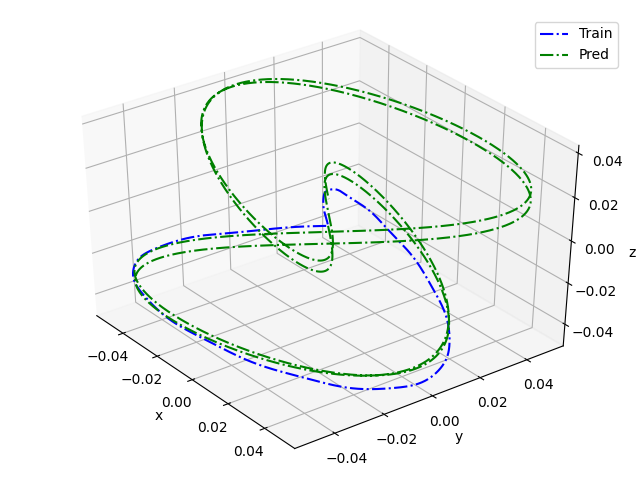
\includegraphics[width=0.5\textwidth]{latent_space_sine.png}
	\caption{Training and predicted latent variables of a sinusoidal data set.}
	\vspace{-2ex}
	\label{fig:sine_latent_space}
\end{figure}
We illustrate the representation learning capabilities by considering a simple sine wave as input to the RRKM model and exploring its latent space. Fig.~\ref{fig:sine_latent_space} shows the latent space embedding of the learned sine wave and evolution of forecasted latent variables. Dynamics in the data are well represented in the latent space and the forecasted latent variables continue to follow the training trajectory. In Fig.~\ref{fig:ablation}, we perform an ablation study on the Santa Fe data set to identify the effect of hyper-parameters on the forecasting performance. We vary bandwidths $\sigma_x , \sigma_t$ and latent-space dimension $s$. The study shows that $\sigma_t$ captures phase-shift, $\sigma_x$ captures amplitude and $s$ capture higher and lower frequencies.

The proposed model is compared to a recurrent neural network (RNN) and an ARMA model which are two of the most popular methods used in time series forecasting. On each data set \footnote{
	\url{https://rdrr.io/cran/TSPred/man/SantaFe.A.html}, \\
	\url{https://archive.ics.uci.edu/ml/datasets/Hungarian+Chickenpox+Cases},\\
	\url{https://archive.ics.uci.edu/ml/datasets/Appliances+energy+prediction},\\
	\url{https://archive.ics.uci.edu/ml/datasets/Gas+Turbine+CO+and+NOx+Emission+Data+Set}.
}, and method, hyperparameter tuning has been performed and the result of the best set of parameters, quantified as the mean squared error, is shown in Table \ref{table:experiment_results}. For all methods, the entire validation set is forecasted, in recursive fashion, starting from the end of the training set.

When comparing to the baseline methods, RRKM is comparable or better. The RNN can have a better result, however, due to its stochastic nature, its performance has high variability while the RRKM is deterministic for the same parameters.

\begin{figure}[!ht]
	\vspace{-2ex}
	\centering
	\setlength\tabcolsep{0pt}
	\def\arraystretch{0.0}%  1 is the default, change whatever you need
	\begin{tabular}{c c}
		\raisebox{-.5\height}{$\sigma_x$} & \raisebox{-.5\height}{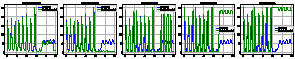
\includegraphics[width=\textwidth]{sigma_x.pdf}}  \\
		\raisebox{-.5\height}{$\sigma_t$} & \raisebox{-.5\height}{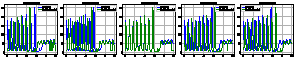
\includegraphics[width=\textwidth]{sigma_t.pdf} } \\
		\raisebox{-.5\height}{$s$}        & \raisebox{-.5\height}{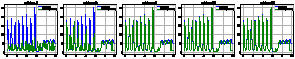
\includegraphics[width=\textwidth]{s.pdf}}
	\end{tabular}
	\vspace{-2ex}
	\caption{Ablation study on the Santa Fe laser data set.\label{fig:ablation}}
\end{figure}

\begin{table}[h]
	\vspace{-2ex}
	\caption{Mean squared error on the forecasted data. Standard deviation for 10 iterations between brackets for the stochastic models.}
	\label{table:experiment_results}
	\centering
	\begin{tabular}{l l l l l}
		\textbf{Data} & \multicolumn{1}{c}{\textbf{RNN}} & \multicolumn{1}{c}{\textbf{ARMA}} & \multicolumn{1}{c}{\textbf{RRKM (Ours)}} \\
		\cmidrule(lr){1-1}\cmidrule(lr){2-4}
		Santa Fe      & 3075.06~($\pm$794.10)            & 2224.55                           & \textbf{119.06}                          \\
		Chickenpox    & 34329.95~($\pm$9513.07)          & 23571.35                          & \textbf{20716.91}                        \\
		Energy        & {16002.11}~($\pm$1809.89)        & 24797.40                          & \textbf{12764.097}                       \\
		Turbine       & 2401.12~($\pm$644.53)            & 1317.67                           & \textbf{1299.915}
	\end{tabular}
	\vspace{-2ex}
\end{table}
% 
% 
% \subsection{SantaFe Laser}
% Non-linear Auto-regressive model (NAR):
% 
% \begin{equation}
% 	\hat{y}_{k}=f\big(\hat{y}_{k-1},\hat{y}_{k-2}\dots\hat{y}_{k-p}\big),
% \end{equation}
% where $ p $ is the lag parameter.
\section{Conclusion}
In this work, we introduced the recurrent restricted kernel machine model. This framework provides new insights and ideas for time series modeling including latent space dynamics and a novel forecasting method. For future work, we believe a further exploration of the representation learning capabilities in latent space can provide new ways to interpret the data. Additionally, besides the topics mentioned in this work, the framework can be extended towards other tasks involving time series such as denoising, handling missing values and classification.